\providecommand{\thebibpath}{..}
\makeatletter\def\input@path{{\thebibpath/}{.}}\makeatother
\documentclass[main.tex]{subfiles}
\begin{document}

\section{Optimal Control}

	The field of control theory concerns itself with taking a system, and designing a controller that makes it behave in a desirable way.
	Optimal control lets us formally define a measure of desirability, and find the controller that maximizes that measure.

	In order to apply any control theory, we need a model of the system.
	One way to model dynamical systems is with discrete-time equations, which for a sufficiently small timestep, are close approximations to their continuous-time counterparts.
	For a suitable choice of state vector $\bm{x}$ and timestep $\delta t$, discrete-time systems can be described in terms of the transition dynamics,
	\begin{align}
		\bm{x}\tind{i + 1} = f(\bm{x}\tind{i}, \bm{u}\tind{i}) \quad \text{where} \quad \bm{x}\tind{i} := x(t_0 + i\cdot\delta t)\,. \label{eq:transition}
	\end{align}
	From this, the optimal control problem in discrete time can be stated as
	\begin{alignat}{2}
		\text{find}&& \quad
			\pi^*(\bm{x}) &= \argmin_{\pi(\bm{x})}
				J(\bm{x}\tind\cdot, \bm{u}\tind\cdot)
				\quad \text{where} \quad
				J(\bm{x}\tind\cdot, \bm{u}\tind\cdot) = \sum_{i=0}^{i=N} c(\bm{x}\tind{i}, \bm{u}\tind{i})\quad \\ \label{eq:optimal}
		\text{st.}&& \quad
			\bm{x}\tind{i+1} &= f(\bm{x}\tind{i}, \bm{u}\tind{i}) \\ \nonumber
		&&
			\bm{u}\tind{i} &= \pi(\bm{x}\tind{i})\, \nonumber
	\end{alignat}
	where $\pi(\bm{x})$ is a policy that computes the desired actions for a given state, and $c(\bm{x}, \bm{u})$ attributes a cost to a set of states and actions at a single timestep.

\section{Gaussian Processes}

	\begin{figure}[b]
		\centering
		\begin{subfigure}[t]{0.3\linewidth}
			% This file was created by matlab2tikz.
%
%The latest updates can be retrieved from
%  http://www.mathworks.com/matlabcentral/fileexchange/22022-matlab2tikz-matlab2tikz
%where you can also make suggestions and rate matlab2tikz.
%
\definecolor{mycolor1}{rgb}{0.63500,0.07800,0.18400}%
%
\begin{tikzpicture}[%
trim axis left,
trim axis right
]

\begin{axis}[%
width=0.951\linewidth,
height=3cm,
at={(0\linewidth,0cm)},
scale only axis,
xmin=0,
xmax=4,
xtick={0,0.5,1,1.5,2,2.5,3,3.5,4},
xticklabels={{}},
xlabel style={font=\color{white!15!black}},
xlabel={$x$},
ymin=0,
ymax=0.8,
ytick={0,0.1,0.2,0.3,0.4,0.5,0.6,0.7,0.8},
yticklabels={{}},
ylabel style={font=\color{white!15!black}},
ylabel={$p(x; \mu, \sigma)$},
axis background/.style={fill=white},
axis x line*=bottom,
axis y line*=left
]

\addplot[area legend, draw=none, fill=gray, fill opacity=0.5, forget plot]
table[row sep=crcr] {%
x	y\\
1.17757318652426	0\\
1.17757318652426	0.206271280750742\\
1.19418786962478	0.217739097897359\\
1.2108025527253	0.229590825441285\\
1.22741723582582	0.241820489345824\\
1.24403191892634	0.254420509452383\\
1.26064660202686	0.267381648294113\\
1.27726128512738	0.280692966593307\\
1.2938759682279	0.294341786092705\\
1.31049065132842	0.308313660346281\\
1.32710533442894	0.322592354063595\\
1.34372001752946	0.337159831563359\\
1.36033470062998	0.351996254846595\\
1.3769493837305	0.367079991747673\\
1.39356406683102	0.382387634562911\\
1.41017874993154	0.397894029491587\\
1.42679343303206	0.413572317153464\\
1.44340811613258	0.429393984370811\\
1.4600227992331	0.445328927321905\\
1.47663748233362	0.461345526087756\\
1.49325216543414	0.47741073052501\\
1.50986684853466	0.493490157306383\\
1.52648153163518	0.509548197876469\\
1.5430962147357	0.52554813697604\\
1.55971089783622	0.541452281293194\\
1.57632558093674	0.557222097705589\\
1.59294026403726	0.572818360485709\\
1.60955494713778	0.588201306751485\\
1.6261696302383	0.603330799358753\\
1.64278431333882	0.618166496350794\\
1.65939899643934	0.632668026004713\\
1.67601367953986	0.646795166445348\\
1.69262836264038	0.660508028735915\\
1.7092430457409	0.673767242301157\\
1.72585772884142	0.686534141494462\\
1.74247241194194	0.69877095208558\\
1.75908709504246	0.710440976420969\\
1.77570177814298	0.721508775994845\\
1.7923164612435	0.731940350165936\\
1.80893114434402	0.74170330976318\\
1.82554582744454	0.750767044343062\\
1.84216051054506	0.759102881892104\\
1.85877519364558	0.766684239809985\\
1.8753898767461	0.773486766061606\\
1.89200455984662	0.779488469449809\\
1.90861924294714	0.784669838033812\\
1.92523392604766	0.789013944801169\\
1.94184860914818	0.792506539792436\\
1.9584632922487	0.795136127976925\\
1.97507797534922	0.796894032283945\\
1.99169265844974	0.797774441305843\\
2.00830734155026	0.797774441305843\\
2.02492202465078	0.796894032283945\\
2.0415367077513	0.795136127976925\\
2.05815139085182	0.792506539792436\\
2.07476607395234	0.789013944801169\\
2.09138075705286	0.784669838033812\\
2.10799544015338	0.779488469449809\\
2.1246101232539	0.773486766061606\\
2.14122480635442	0.766684239809985\\
2.15783948945494	0.759102881892104\\
2.17445417255546	0.750767044343062\\
2.19106885565598	0.74170330976318\\
2.2076835387565	0.731940350165936\\
2.22429822185702	0.721508775994845\\
2.24091290495754	0.710440976420969\\
2.25752758805806	0.69877095208558\\
2.27414227115858	0.686534141494462\\
2.2907569542591	0.673767242301157\\
2.30737163735962	0.660508028735915\\
2.32398632046014	0.646795166445348\\
2.34060100356066	0.632668026004713\\
2.35721568666118	0.618166496350794\\
2.3738303697617	0.603330799358753\\
2.39044505286222	0.588201306751485\\
2.40705973596274	0.572818360485709\\
2.42367441906326	0.557222097705589\\
2.44028910216378	0.541452281293194\\
2.4569037852643	0.52554813697604\\
2.47351846836482	0.509548197876469\\
2.49013315146534	0.493490157306383\\
2.50674783456586	0.47741073052501\\
2.52336251766638	0.461345526087757\\
2.5399772007669	0.445328927321905\\
2.55659188386742	0.429393984370811\\
2.57320656696794	0.413572317153464\\
2.58982125006846	0.397894029491587\\
2.60643593316898	0.382387634562911\\
2.6230506162695	0.367079991747673\\
2.63966529937002	0.351996254846596\\
2.65627998247054	0.337159831563359\\
2.67289466557106	0.322592354063595\\
2.68950934867158	0.308313660346281\\
2.7061240317721	0.294341786092705\\
2.72273871487262	0.280692966593307\\
2.73935339797314	0.267381648294114\\
2.75596808107366	0.254420509452383\\
2.77258276417418	0.241820489345824\\
2.7891974472747	0.229590825441285\\
2.80581213037522	0.217739097897359\\
2.82242681347574	0.206271280750742\\
2.82242681347574	0\\
}--cycle;
\addplot [color=black, forget plot]
  table[row sep=crcr]{%
0	0.000267660451529771\\
0.0404040404040404	0.000368590604636303\\
0.0808080808080808	0.000504276112305317\\
0.121212121212121	0.000685419745917184\\
0.161616161616162	0.0009255692289194\\
0.202020202020202	0.00124172459833281\\
0.242424242424242	0.00165502950936388\\
0.282828282828283	0.00219154442862412\\
0.323232323232323	0.00288309463307419\\
0.363636363636364	0.00376817962030763\\
0.404040404040404	0.00489292293663676\\
0.444444444444444	0.00631203263283609\\
0.484848484848485	0.00808973277177296\\
0.525252525252525	0.0103006159847218\\
0.565656565656566	0.0130303565045358\\
0.606060606060606	0.0163762130535745\\
0.646464646464647	0.0204472422439212\\
0.686868686868687	0.0253641366983196\\
0.727272727272727	0.0312585989537112\\
0.767676767676768	0.0382721634279922\\
0.808080808080808	0.0465543853321692\\
0.848484848484849	0.0562603282745569\\
0.888888888888889	0.0675473020705413\\
0.929292929292929	0.0805708292326468\\
0.96969696969697	0.0954798526137071\\
1.01010101010101	0.112411237017888\\
1.05050505050505	0.131483662992913\\
1.09090909090909	0.152791059570133\\
1.13131313131313	0.176395771937897\\
1.17171717171717	0.202321706924249\\
1.21212121212121	0.230547740368852\\
1.25252525252525	0.261001702453701\\
1.29292929292929	0.293555276383304\\
1.33333333333333	0.328020149351987\\
1.37373737373737	0.364145740040454\\
1.41414141414141	0.401618792392587\\
1.45454545454545	0.440065070739981\\
1.4949494949495	0.47905331740255\\
1.53535353535354	0.518101543059398\\
1.57575757575758	0.556685616223426\\
1.61616161616162	0.594250006109949\\
1.65656565656566	0.63022041913464\\
1.6969696969697	0.664017959950017\\
1.73737373737374	0.695074350302397\\
1.77777777777778	0.722847659765487\\
1.81818181818182	0.746837947507958\\
1.85858585858586	0.76660218834497\\
1.8989898989899	0.781767862399903\\
1.93939393939394	0.792044626781266\\
1.97979797979798	0.797233558647621\\
2.02020202020202	0.797233558647621\\
2.06060606060606	0.792044626781266\\
2.1010101010101	0.781767862399903\\
2.14141414141414	0.76660218834497\\
2.18181818181818	0.746837947507958\\
2.22222222222222	0.722847659765487\\
2.26262626262626	0.695074350302397\\
2.3030303030303	0.664017959950017\\
2.34343434343434	0.63022041913464\\
2.38383838383838	0.594250006109949\\
2.42424242424242	0.556685616223426\\
2.46464646464646	0.518101543059399\\
2.50505050505051	0.47905331740255\\
2.54545454545455	0.440065070739981\\
2.58585858585859	0.401618792392587\\
2.62626262626263	0.364145740040454\\
2.66666666666667	0.328020149351987\\
2.70707070707071	0.293555276383304\\
2.74747474747475	0.261001702453701\\
2.78787878787879	0.230547740368851\\
2.82828282828283	0.202321706924249\\
2.86868686868687	0.176395771937898\\
2.90909090909091	0.152791059570133\\
2.94949494949495	0.131483662992913\\
2.98989898989899	0.112411237017888\\
3.03030303030303	0.0954798526137071\\
3.07070707070707	0.0805708292326469\\
3.11111111111111	0.0675473020705413\\
3.15151515151515	0.0562603282745569\\
3.19191919191919	0.0465543853321692\\
3.23232323232323	0.0382721634279922\\
3.27272727272727	0.0312585989537112\\
3.31313131313131	0.0253641366983196\\
3.35353535353535	0.0204472422439212\\
3.39393939393939	0.0163762130535745\\
3.43434343434343	0.0130303565045358\\
3.47474747474747	0.0103006159847218\\
3.51515151515152	0.00808973277177296\\
3.55555555555556	0.0063120326328361\\
3.5959595959596	0.00489292293663676\\
3.63636363636364	0.00376817962030763\\
3.67676767676768	0.00288309463307418\\
3.71717171717172	0.00219154442862412\\
3.75757575757576	0.00165502950936388\\
3.7979797979798	0.00124172459833281\\
3.83838383838384	0.000925569228919402\\
3.87878787878788	0.000685419745917184\\
3.91919191919192	0.000504276112305317\\
3.95959595959596	0.000368590604636302\\
4	0.000267660451529771\\
};
\addplot [color=mycolor1, draw=none, mark=o, mark options={solid, mycolor1}, forget plot]
  table[row sep=crcr]{%
2.10486214487437	0\\
2.3174485110034	0\\
2.5311903994273	0\\
2.89462424982559	0\\
2.11384782642133	0\\
1.86481982768848	0\\
1.47056427896252	0\\
1.88559118455983	0\\
1.54873259527504	0\\
1.55799539691512	0\\
};
\end{axis}
\end{tikzpicture}%
			\caption{1D Gaussian distribution}
			\label{fig:gaussian:1d}
		\end{subfigure}%
		\hfill
		\begin{subfigure}[t]{0.3\linewidth}
			% This file was created by matlab2tikz.
%
%The latest updates can be retrieved from
%  http://www.mathworks.com/matlabcentral/fileexchange/22022-matlab2tikz-matlab2tikz
%where you can also make suggestions and rate matlab2tikz.
%
\definecolor{mycolor1}{rgb}{0.63500,0.07800,0.18400}%
%
\begin{tikzpicture}[%
trim axis left,
trim axis right
]

\begin{axis}[%
width=0.951\linewidth,
height=3cm,
at={(0\linewidth,0cm)},
scale only axis,
xmin=-0.978366170242519,
xmax=2.82531481135257,
xtick={-2,-1.5,-1,-0.5,0,0.5,1,1.5,2},
xticklabels={{}},
xlabel style={font=\color{white!15!black}},
xlabel={$x_1$},
ymin=0.5,
ymax=3.5,
ytick={-1,-0.5,0,0.5,1,1.5,2,2.5,3},
yticklabels={{}},
ylabel style={font=\color{white!15!black}},
ylabel={$x_2$},
axis background/.style={fill=white},
axis x line*=bottom,
axis y line*=left
]

\addplot[area legend, draw=none, fill=gray, fill opacity=0.5, forget plot]
table[row sep=crcr] {%
x	y\\
0.768979372139707	1.23699069848947\\
0.726730020205697	1.25019378682406\\
0.68475035274946	1.26413684336585\\
0.643081798634509	1.2788061080014\\
0.601765479693048	1.29418710393756\\
0.560842170143694	1.31026465198831\\
0.52035225635224	1.32702288555479\\
0.480335696975194	1.34444526628371\\
0.440831983525401	1.36251460038874\\
0.401880101398695	1.38121305561863\\
0.363518491400019	1.40052217885557\\
0.325785011806987	1.42042291432615\\
0.28871690100834	1.4408956224071\\
0.252350740754148	1.46192009900724\\
0.216722420054043	1.48347559550649\\
0.181867099759096	1.50554083923223\\
0.147819177862305	1.52809405445287\\
0.114612255551927	1.55111298386787\\
0.0822791040511605	1.574574910573\\
0.0508516322769095	1.59845668047921\\
0.0203608553495296	1.62273472516287\\
-0.00916313601534702	1.647385085125\\
-0.0376912052027187	1.67238343343641\\
-0.0651951984525325	1.69770509974538\\
-0.0916479726440491	1.7233250946244\\
-0.117023422082822	1.74921813423166\\
-0.141296504263872	1.77535866526317\\
-0.16444326458561	1.80172089017078\\
-0.186440859990141	1.82827879262128\\
-0.207267581506603	1.8550061631713\\
-0.2269028756753	1.88187662513295\\
-0.245327364831484	1.9088636606044\\
-0.262522866228774	1.9359406366398\\
-0.278472409983329	1.96308083153285\\
-0.293160255821075	1.99025746118788\\
-0.306571908611456	2.01744370555249\\
-0.318694132672375	2.04461273508571\\
-0.329514964832219	2.07173773723557\\
-0.33902372623606	2.09879194289978\\
-0.3472110328844	2.12574865284365\\
-0.354068804894042	2.15258126404898\\
-0.359590274471962	2.17926329596804\\
-0.363769992594301	2.20576841665671\\
-0.366603834383896	2.23207046876086\\
-0.368089003181034	2.25814349533055\\
-0.36822403330342	2.2839617654364\\
-0.367008791492625	2.30949979956287\\
-0.364444477045598	2.33473239475354\\
-0.360533620631105	2.35963464948332\\
-0.355280081792263	2.38418198823328\\
-0.34868904513764	2.4083501857437\\
-0.340767015224668	2.43211539092152\\
-0.331521810140432	2.45545415037841\\
-0.320962553786165	2.47834343157653\\
-0.309099666873052	2.50076064555878\\
-0.295944856638253	2.52268366924143\\
-0.281511105291272	2.54409086724691\\
-0.265812657202078	2.5649611132553\\
-0.248865004843641	2.58527381085349\\
-0.230684873502721	2.60500891386133\\
-0.21129020477404	2.6241469461148\\
-0.190700138854086	2.64266902068663\\
-0.168934995652053	2.66055685852541\\
-0.146016254736543	2.67779280649482\\
-0.121966534137828	2.69435985479514\\
-0.0968095680265795	2.71024165374986\\
-0.0705701832911125	2.72542252994084\\
-0.0432742750362425	2.73988750167609\\
-0.0149487810279409	2.75362229377489\\
0.0143783448909837	2.76661335165566\\
0.0446781603879562	2.77884785471269\\
0.0759207632032231	2.79031372896856\\
0.108075320659769	2.80099965898968\\
0.141110100091454	2.81089509905323\\
0.174992500159313	2.81999028355457\\
0.209689083025152	2.82827623664466\\
0.245165607350653	2.83574478108819\\
0.281387062089437	2.84238854633348\\
0.318317701038748	2.84820097578634\\
0.355921078116633	2.85317633328064\\
0.394160083329825	2.85730970873921\\
0.432996979396832	2.86059702301952\\
0.472393438990069	2.86303503193925\\
0.512310582560312	2.86462132947794\\
0.55270901670611	2.86535435015142\\
0.593548873050325	2.86523337055681\\
0.6347898475854	2.86425851008635\\
0.676391240448551	2.86243073080962\\
0.718311996087622	2.85975183652411\\
0.760510743777949	2.85622447097505\\
0.802945838450278	2.85185211524637\\
0.84557540178942	2.84663908432529\\
0.888357363563088	2.84059052284396\\
0.931249503140141	2.83371240000231\\
0.974209491157246	2.82601150367717\\
1.01719493129285	2.81749543372348\\
1.06016340210724	2.80817259447413\\
1.10307249890737	2.79805218644588\\
1.14587987559517	2.78714419725963\\
1.18854328645804	2.77545939178375\\
1.23102062786029	2.76300930151053\\
1.2732699797943	2.74980621317594\\
1.31524964725054	2.73586315663415\\
1.35691820136549	2.7211938919986\\
1.39823452030695	2.70581289606244\\
1.43915782985631	2.68973534801169\\
1.47964774364776	2.67297711444521\\
1.51966430302481	2.65555473371629\\
1.5591680164746	2.63748539961126\\
1.5981198986013	2.61878694438137\\
1.63648150859998	2.59947782114443\\
1.67421498819301	2.57957708567385\\
1.71128309899166	2.5591043775929\\
1.74764925924585	2.53807990099276\\
1.78327757994596	2.51652440449351\\
1.8181329002409	2.49445916076777\\
1.85218082213769	2.47190594554713\\
1.88538774444807	2.44888701613213\\
1.91772089594884	2.425425089427\\
1.94914836772309	2.40154331952079\\
1.97963914465047	2.37726527483713\\
2.00916313601535	2.352614914875\\
2.03769120520272	2.3276165665636\\
2.06519519845253	2.30229490025462\\
2.09164797264405	2.2766749053756\\
2.11702342208282	2.25078186576834\\
2.14129650426387	2.22464133473683\\
2.16444326458561	2.19827910982922\\
2.18644085999014	2.17172120737872\\
2.2072675815066	2.1449938368287\\
2.2269028756753	2.11812337486705\\
2.24532736483148	2.0911363393956\\
2.26252286622877	2.0640593633602\\
2.27847240998333	2.03691916846715\\
2.29316025582107	2.00974253881212\\
2.30657190861146	1.98255629444751\\
2.31869413267238	1.95538726491429\\
2.32951496483222	1.92826226276443\\
2.33902372623606	1.90120805710022\\
2.3472110328844	1.87425134715635\\
2.35406880489404	1.84741873595103\\
2.35959027447196	1.82073670403196\\
2.3637699925943	1.79423158334329\\
2.3666038343839	1.76792953123914\\
2.36808900318103	1.74185650466945\\
2.36822403330342	1.7160382345636\\
2.36700879149262	1.69050020043713\\
2.3644444770456	1.66526760524646\\
2.3605336206311	1.64036535051668\\
2.35528008179226	1.61581801176672\\
2.34868904513764	1.5916498142563\\
2.34076701522467	1.56788460907849\\
2.33152181014043	1.54454584962159\\
2.32096255378617	1.52165656842347\\
2.30909966687305	1.49923935444122\\
2.29594485663825	1.47731633075857\\
2.28151110529127	1.45590913275309\\
2.26581265720208	1.4350388867447\\
2.24886500484364	1.41472618914651\\
2.23068487350272	1.39499108613867\\
2.21129020477404	1.3758530538852\\
2.19070013885409	1.35733097931338\\
2.16893499565205	1.33944314147459\\
2.14601625473654	1.32220719350518\\
2.12196653413783	1.30564014520486\\
2.09680956802658	1.28975834625014\\
2.07057018329111	1.27457747005916\\
2.04327427503624	1.26011249832391\\
2.01494878102794	1.24637770622511\\
1.98562165510902	1.23338664834434\\
1.95532183961204	1.22115214528731\\
1.92407923679678	1.20968627103144\\
1.89192467934023	1.19900034101032\\
1.85888989990855	1.18910490094677\\
1.82500749984069	1.18000971644543\\
1.79031091697485	1.17172376335534\\
1.75483439264935	1.16425521891181\\
1.71861293791056	1.15761145366652\\
1.68168229896125	1.15179902421366\\
1.64407892188337	1.14682366671936\\
1.60583991667018	1.14269029126079\\
1.56700302060317	1.13940297698048\\
1.52760656100993	1.13696496806075\\
1.48768941743969	1.13537867052207\\
1.44729098329389	1.13464564984858\\
1.40645112694968	1.13476662944319\\
1.3652101524146	1.13574148991365\\
1.32360875955145	1.13756926919038\\
1.28168800391238	1.14024816347589\\
1.23948925622205	1.14377552902495\\
1.19705416154972	1.14814788475363\\
1.15442459821058	1.15336091567471\\
1.11164263643691	1.15940947715604\\
1.06875049685986	1.16628759999769\\
1.02579050884275	1.17398849632283\\
0.982805068707147	1.18250456627652\\
0.939836597892757	1.19182740552587\\
0.896927501092631	1.20194781355412\\
0.854120124404832	1.21285580274037\\
0.811456713541956	1.22454060821625\\
0.768979372139707	1.23699069848947\\
}--cycle;
\addplot [color=mycolor1, draw=none, mark=o, mark options={solid, mycolor1}, forget plot]
  table[row sep=crcr]{%
1.62168985772206	1.23319741840057\\
-0.587602734884004	2.69550462158856\\
0.654412359379664	2.24916339882187\\
0.212027330163576	2.40979113724902\\
2.23708595224499	1.39906225859969\\
0.949399287486024	2.13161156498154\\
0.47402533634125	2.48475995719116\\
0.804673942880572	2.12421668460537\\
0.419678263290235	2.4155337431119\\
0.870160557857379	2.05692839835231\\
0.564588505601391	2.22420707552924\\
1.29124732916342	2.18692999207973\\
1.31507621361342	1.60279946697807\\
1.3035525493338	2.31257712708344\\
1.1495798927265	1.80744863845831\\
0.371725611929442	2.33558117665467\\
1.12732693572524	1.67585886862615\\
1.22697793180628	1.69968063090332\\
0.0791835638554578	1.98103195915242\\
1.44121236292173	2.10265261413699\\
1.18517475716689	1.4187349367444\\
1.50343148953022	1.77117958688951\\
1.34789370954102	1.73144646175673\\
0.786613620468095	2.27584290790401\\
2.43455137599406	2.06388386700375\\
1.2134890945905	2.03443026268702\\
1.0611784032452	2.0205199638735\\
0.731083846566839	1.40104149090502\\
1.94552345481951	2.13883935233326\\
0.479603449359114	1.88512026660411\\
1.34791998024851	1.86675300099744\\
1.13337542611373	1.81614086588043\\
1.74514836450965	2.67761202921273\\
2.39595683555146	1.53478272330273\\
1.63727722223667	1.788012157073\\
1.17040538445556	2.25348062671072\\
1.03627772619526	1.72185695316155\\
1.36779663288073	2.10449285814305\\
1.01674936612708	1.84654258927429\\
1.43491401911157	2.29499423790677\\
1.60619456014794	2.13429642639953\\
1.11386864264935	3.11900306041096\\
1.25526263382011	2.07473885125444\\
1.02230851133055	2.0176376482359\\
1.55887259687329	1.42871807096233\\
-0.238078139405796	2.42282794792377\\
0.800094693378852	2.15817667293352\\
0.726871306657918	2.41303519150767\\
0.555644195614291	2.14916985224035\\
0.842651423931794	1.88818962077398\\
};
\end{axis}
\end{tikzpicture}%
			\caption{2D Gaussian distribution}
			\label{fig:gaussian:2d}
		\end{subfigure}%
		\hfill
		\begin{subfigure}[t]{0.3\linewidth}
			% This file was created by matlab2tikz.
%
%The latest updates can be retrieved from
%  http://www.mathworks.com/matlabcentral/fileexchange/22022-matlab2tikz-matlab2tikz
%where you can also make suggestions and rate matlab2tikz.
%
\definecolor{mycolor1}{rgb}{0.63500,0.07800,0.18400}%
%
\begin{tikzpicture}[%
trim axis left,
trim axis right
]

\begin{axis}[%
width=0.951\linewidth,
height=3cm,
at={(0\linewidth,0cm)},
scale only axis,
xmin=0,
xmax=4,
xtick={0,0.5,1,1.5,2,2.5,3,3.5,4},
xticklabels={{}},
xlabel style={font=\color{white!15!black}},
xlabel={$i$},
ymin=-2,
ymax=2,
ytick={-2,-1.5,-1,-0.5,0,0.5,1,1.5,2},
yticklabels={{}},
ylabel style={font=\color{white!15!black}},
ylabel={$x(i)$},
axis background/.style={fill=white},
axis x line*=bottom,
axis y line*=left
]

\addplot[area legend, draw=none, fill=gray, fill opacity=0.5, forget plot]
table[row sep=crcr] {%
x	y\\
0	1.33894093138436\\
0.0404040404040404	1.30759268640533\\
0.0808080808080808	1.27416049771751\\
0.121212121212121	1.23860882221759\\
0.161616161616162	1.20091109390162\\
0.202020202020202	1.1610503566414\\
0.242424242424242	1.1190198386713\\
0.282828282828283	1.07482346168818\\
0.323232323232323	1.02847627816469\\
0.363636363636364	0.980004831260679\\
0.404040404040404	0.929447432576734\\
0.444444444444444	0.876854353916285\\
0.484848484848485	0.822287930194645\\
0.525252525252525	0.765822571640604\\
0.565656565656566	0.707544684463923\\
0.606060606060606	0.647552500194751\\
0.646464646464647	0.585955814922915\\
0.686868686868687	0.522875640660376\\
0.727272727272727	0.458443772003447\\
0.767676767676768	0.392802272167531\\
0.808080808080808	0.326102883292137\\
0.848484848484849	0.258506366654687\\
0.888888888888889	0.190181779076716\\
0.929292929292929	0.121305692345679\\
0.96969696969697	0.0520613629021163\\
1.01010101010101	0.0145991338972249\\
1.05050505050505	0.0723766497107184\\
1.09090909090909	0.129003620555568\\
1.13131313131313	0.18426700099537\\
1.17171717171717	0.237955319599258\\
1.21212121212121	0.289859890086144\\
1.25252525252525	0.339776008540474\\
1.29292929292929	0.38750412781218\\
1.33333333333333	0.432851000681895\\
1.37373737373737	0.475630783918306\\
1.41414141414141	0.515666095962986\\
1.45454545454545	0.55278902163469\\
1.4949494949495	0.586842057934705\\
1.53535353535354	0.617678995741859\\
1.57575757575758	0.645165732895641\\
1.61616161616162	0.669181014864292\\
1.65656565656566	0.68961709986907\\
1.6969696969697	0.706380345974817\\
1.73737373737374	0.719391718251518\\
1.77777777777778	0.728587214654395\\
1.81818181818182	0.733918209756796\\
1.85858585858586	0.735351715898536\\
1.8989898989899	0.732870561682673\\
1.93939393939394	0.72647348806883\\
1.97979797979798	0.716175162576002\\
2.02020202020202	0.702006112329395\\
2.06060606060606	0.684012576872861\\
2.1010101010101	0.662256281830744\\
2.14141414141414	0.63681413465141\\
2.18181818181818	0.607777843810091\\
2.22222222222222	0.575253463002362\\
2.26262626262626	0.539360862031278\\
2.3030303030303	0.500233126290724\\
2.34343434343434	0.458015886982118\\
2.38383838383838	0.412866584477157\\
2.42424242424242	0.364953667559814\\
2.46464646464646	0.314455731647025\\
2.50505050505051	0.26156059949887\\
2.54545454545455	0.206464348381622\\
2.58585858585859	0.14937028813506\\
2.62626262626263	0.0904878951105028\\
2.66666666666667	0.0300317074782748\\
2.70707070707071	-0.0317798120592501\\
2.74747474747475	-0.0947254395834641\\
2.78787878787879	-0.158582372230257\\
2.82828282828283	-0.223127421870649\\
2.86868686868687	-0.288138212233831\\
2.90909090909091	-0.353394371148582\\
2.94949494949495	-0.418678709298082\\
2.98989898989899	-0.483778376691341\\
3.03030303030303	-0.452309101810315\\
3.07070707070707	-0.387740244453384\\
3.11111111111111	-0.322239400460619\\
3.15151515151515	-0.256012423402569\\
3.19191919191919	-0.1892636024007\\
3.23232323232323	-0.122194577988257\\
3.27272727272727	-0.0550032802017414\\
3.31313131313131	0.0121171015161398\\
3.35353535353535	0.0789791072211162\\
3.39393939393939	0.145401945135791\\
3.43434343434343	0.211212371510147\\
3.47474747474747	0.276245503699543\\
3.51515151515152	0.34034555920001\\
3.55555555555556	0.403366514202103\\
3.5959595959596	0.465172676138444\\
3.63636363636364	0.52563916569356\\
3.67676767676768	0.584652304801634\\
3.71717171717172	0.642109908262576\\
3.75757575757576	0.697921477741728\\
3.7979797979798	0.752008298067845\\
3.83838383838384	0.804303436889115\\
3.87878787878788	0.854751649872262\\
3.91919191919192	0.903309194717945\\
3.95959595959596	0.94994355830152\\
4	0.99463310221609\\
4	-1.62056574492566\\
3.95959595959596	-1.60014864510581\\
3.91919191919192	-1.57768008100027\\
3.87878787878788	-1.55309506793653\\
3.83838383838384	-1.52633699011473\\
3.7979797979798	-1.49735844251796\\
3.75757575757576	-1.46612202552858\\
3.71717171717172	-1.4326010830895\\
3.67676767676768	-1.39678037574202\\
3.63636363636364	-1.35865668047412\\
3.5959595959596	-1.31823931001742\\
3.55555555555556	-1.27555054502897\\
3.51515151515152	-1.23062597347478\\
3.47474747474747	-1.1835147324855\\
3.43434343434343	-1.13427964896632\\
3.39393939393939	-1.08299727630139\\
3.35353535353535	-1.02975782558188\\
3.31313131313131	-0.974664990891168\\
3.27272727272727	-0.917835669285202\\
3.23232323232323	-0.85939957719499\\
3.19191919191919	-0.799498766034983\\
3.15151515151515	-0.738287040810975\\
3.11111111111111	-0.675929286470618\\
3.07070707070707	-0.612600707613061\\
3.03030303030303	-0.548485987961175\\
2.98989898989899	-0.51573965123878\\
2.94949494949495	-0.577826203477327\\
2.90909090909091	-0.638364794722935\\
2.86868686868687	-0.697154264729565\\
2.82828282828283	-0.753997311032638\\
2.78787878787879	-0.808701511331117\\
2.74747474747475	-0.861080306726273\\
2.70707070707071	-0.910953939265186\\
2.66666666666667	-0.958150338048989\\
2.62626262626263	-1.00250594902311\\
2.58585858585859	-1.0438665044481\\
2.54545454545455	-1.08208772893851\\
2.50505050505051	-1.11703597983099\\
2.46464646464646	-1.1485888204854\\
2.42424242424242	-1.17663552591466\\
2.38383838383838	-1.20107752086529\\
2.34343434343434	-1.22182875111745\\
2.3030303030303	-1.23881598932836\\
2.26262626262626	-1.25197907719923\\
2.22222222222222	-1.26127110609627\\
2.18181818181818	-1.26665853850048\\
2.14141414141414	-1.2681212727979\\
2.1010101010101	-1.26565265395838\\
2.06060606060606	-1.25925943259261\\
2.02020202020202	-1.24896167473509\\
1.97979797979798	-1.23479262448848\\
1.93939393939394	-1.21679852139665\\
1.8989898989899	-1.19503837410645\\
1.85858585858586	-1.16958369155077\\
1.81818181818182	-1.14051817255378\\
1.77777777777778	-1.10793735444424\\
1.73737373737374	-1.07194822097898\\
1.6969696969697	-1.03266876964427\\
1.65656565656566	-0.990227538230495\\
1.61616161616162	-0.944763090478155\\
1.57575757575758	-0.896423460578834\\
1.53535353535354	-0.845365556390569\\
1.4949494949495	-0.791754521395153\\
1.45454545454545	-0.735763055685444\\
1.41414141414141	-0.677570696620178\\
1.37373737373737	-0.617363060215303\\
1.33333333333333	-0.555331044845371\\
1.29292929292929	-0.491669999393737\\
1.25252525252525	-0.426578858602334\\
1.21212121212121	-0.360259249014704\\
1.17171717171717	-0.292914569562722\\
1.13131313131313	-0.224749051500359\\
1.09090909090909	-0.155966803018742\\
1.05050505050505	-0.0867708444685266\\
1.01010101010101	-0.0173621406503643\\
0.96969696969697	-0.0441155232487941\\
0.929292929292929	-0.103554770813987\\
0.888888888888889	-0.163508106933296\\
0.848484848484849	-0.223768250753692\\
0.808080808080808	-0.28413228034215\\
0.767676767676768	-0.344402727039222\\
0.727272727272727	-0.404388617079996\\
0.686868686868687	-0.463906451746933\\
0.646464646464647	-0.522781117880096\\
0.606060606060606	-0.580846721242423\\
0.565656565656566	-0.637947336012539\\
0.525252525252525	-0.693937664544437\\
0.484848484848485	-0.748683602480138\\
0.444444444444444	-0.802062705314783\\
0.404040404040404	-0.853964553579141\\
0.363636363636364	-0.904291014907002\\
0.323232323232323	-0.952956402378972\\
0.282828282828283	-0.999887529663901\\
0.242424242424242	-1.04502366459901\\
0.202020202020202	-1.08831638394441\\
0.161616161616162	-1.12972933310222\\
0.121212121212121	-1.1692378955912\\
0.0808080808080808	-1.20682877800071\\
0.0404040404040404	-1.24249951700201\\
0	-1.27625791575739\\
}--cycle;
\addplot [color=mycolor1, forget plot]
  table[row sep=crcr]{%
0	0.478469582417546\\
0.0404040404040404	0.457518910022232\\
0.0808080808080808	0.433492092958278\\
0.121212121212121	0.407088662415206\\
0.161616161616162	0.379731942281659\\
0.202020202020202	0.349658076412809\\
0.242424242424242	0.318887634555395\\
0.282828282828283	0.288070363788865\\
0.323232323232323	0.255910086724378\\
0.363636363636364	0.224134578367703\\
0.404040404040404	0.193852043804622\\
0.444444444444444	0.163914909263444\\
0.484848484848485	0.134931835427498\\
0.525252525252525	0.107291352594057\\
0.565656565656566	0.0822667579459298\\
0.606060606060606	0.0602578875944031\\
0.646464646464647	0.0402301694923436\\
0.686868686868687	0.0229658269354559\\
0.727272727272727	0.00842623195449402\\
0.767676767676768	-0.00285947541326662\\
0.808080808080808	-0.0102504319901325\\
0.848484848484849	-0.0144095723270378\\
0.888888888888889	-0.0158047765496966\\
0.929292929292929	-0.0123358334269094\\
0.96969696969697	-0.00634395976973593\\
1.01010101010101	0.00322018711850536\\
1.05050505050505	0.0152144225269035\\
1.09090909090909	0.0304199513607418\\
1.13131313131313	0.0480823714583319\\
1.17171717171717	0.0686693226052524\\
1.21212121212121	0.0921542819127697\\
1.25252525252525	0.116798647262324\\
1.29292929292929	0.143813509188276\\
1.33333333333333	0.171857843378672\\
1.37373737373737	0.201280335450405\\
1.41414141414141	0.230998406527799\\
1.45454545454545	0.261173673374284\\
1.4949494949495	0.291439022678276\\
1.53535353535354	0.322230743570669\\
1.57575757575758	0.351545286968389\\
1.61616161616162	0.37964692360427\\
1.65656565656566	0.406855452959618\\
1.6969696969697	0.432188700595606\\
1.73737373737374	0.455575945253821\\
1.77777777777778	0.476804042959088\\
1.81818181818182	0.495229853362924\\
1.85858585858586	0.511048227421426\\
1.8989898989899	0.522791438365154\\
1.93939393939394	0.531306647255465\\
1.97979797979798	0.536846921019509\\
2.02020202020202	0.537736044116635\\
2.06060606060606	0.534913075105064\\
2.1010101010101	0.527757845164547\\
2.14141414141414	0.516487946938664\\
2.18181818181818	0.500372710062048\\
2.22222222222222	0.480921940283368\\
2.26262626262626	0.455810490697506\\
2.3030303030303	0.427097830404977\\
2.34343434343434	0.393215911114766\\
2.38383838383838	0.356002304585787\\
2.42424242424242	0.314416337825185\\
2.46464646464646	0.269342398259971\\
2.50505050505051	0.220683524810998\\
2.54545454545455	0.168814925707719\\
2.58585858585859	0.11466808036793\\
2.62626262626263	0.0581630886210114\\
2.66666666666667	-0.00185236644286002\\
2.70707070707071	-0.0618686982965438\\
2.74747474747475	-0.123164277871589\\
2.78787878787879	-0.186148778275804\\
2.82828282828283	-0.248284445107553\\
2.86868686868687	-0.309623729627961\\
2.90909090909091	-0.369904581397221\\
2.94949494949495	-0.429372635808935\\
2.98989898989899	-0.486438187773288\\
3.03030303030303	-0.540260392350545\\
3.07070707070707	-0.591511453324493\\
3.11111111111111	-0.639588149711263\\
3.15151515151515	-0.682568865995513\\
3.19191919191919	-0.722291247302741\\
3.23232323232323	-0.756872707532002\\
3.27272727272727	-0.785554842272102\\
3.31313131313131	-0.809318450689232\\
3.35353535353535	-0.827985167063362\\
3.39393939393939	-0.840549698624765\\
3.43434343434343	-0.848018699935092\\
3.47474747474747	-0.84835244467295\\
3.51515151515152	-0.842996604692319\\
3.55555555555556	-0.831497075484333\\
3.5959595959596	-0.814430546181353\\
3.63636363636364	-0.791438256146627\\
3.67676767676768	-0.763256390126166\\
3.71717171717172	-0.730354496508202\\
3.75757575757576	-0.692083074205149\\
3.7979797979798	-0.648936022001407\\
3.83838383838384	-0.60168193635539\\
3.87878787878788	-0.55040277677957\\
3.91919191919192	-0.495945067983782\\
3.95959595959596	-0.438162948673068\\
4	-0.377731363252925\\
};
\addplot [color=mycolor1, forget plot]
  table[row sep=crcr]{%
0	1.60284826614559\\
0.0404040404040404	1.54092822349489\\
0.0808080808080808	1.4731358225784\\
0.121212121212121	1.40044839613468\\
0.161616161616162	1.32471602432669\\
0.202020202020202	1.24622141462148\\
0.242424242424242	1.16435667143981\\
0.282828282828283	1.08184481350115\\
0.323232323232323	0.998448816418469\\
0.363636363636364	0.915146757791022\\
0.404040404040404	0.831705424826958\\
0.444444444444444	0.750355819930581\\
0.484848484848485	0.670776014531228\\
0.525252525252525	0.593878397907915\\
0.565656565656566	0.520626642794438\\
0.606060606060606	0.450259394618403\\
0.646464646464647	0.384006077491542\\
0.686868686868687	0.322450565664098\\
0.727272727272727	0.26483043773382\\
0.767676767676768	0.211160766086137\\
0.808080808080808	0.16358165134981\\
0.848484848484849	0.120481412709561\\
0.888888888888889	0.0821656738820477\\
0.929292929292929	0.0484383412962266\\
0.96969696969697	0.0188799256673567\\
1.01010101010101	-0.0060933697229457\\
1.05050505050505	-0.0264446150206678\\
1.09090909090909	-0.0443120978217886\\
1.13131313131313	-0.058746070668303\\
1.17171717171717	-0.0695444262466091\\
1.21212121212121	-0.0782152791103577\\
1.25252525252525	-0.0850979294556543\\
1.29292929292929	-0.090178985285012\\
1.33333333333333	-0.0940666424420017\\
1.37373737373737	-0.0968727246499494\\
1.41414141414141	-0.0990938355645731\\
1.45454545454545	-0.102456045996181\\
1.4949494949495	-0.106074406078573\\
1.53535353535354	-0.109520613414642\\
1.57575757575758	-0.114709408433973\\
1.61616161616162	-0.120979326212659\\
1.65656565656566	-0.128729805982721\\
1.6969696969697	-0.137693420016658\\
1.73737373737374	-0.150143112853455\\
1.77777777777778	-0.163001248151151\\
1.81818181818182	-0.17754413131811\\
1.85858585858586	-0.194379977244496\\
1.8989898989899	-0.212059037985923\\
1.93939393939394	-0.231600030646979\\
1.97979797979798	-0.253691564613625\\
2.02020202020202	-0.276106373183013\\
2.06060606060606	-0.299419495988814\\
2.1010101010101	-0.323604814967954\\
2.14141414141414	-0.348464954576695\\
2.18181818181818	-0.374084232618906\\
2.22222222222222	-0.399016122031278\\
2.26262626262626	-0.422872637997563\\
2.3030303030303	-0.446540677681178\\
2.34343434343434	-0.469700483957387\\
2.38383838383838	-0.491115513900016\\
2.42424242424242	-0.510291118400803\\
2.46464646464646	-0.527778090031495\\
2.50505050505051	-0.542858715158121\\
2.54545454545455	-0.556226982619163\\
2.58585858585859	-0.567100654918981\\
2.62626262626263	-0.573872157888552\\
2.66666666666667	-0.578975382414508\\
2.70707070707071	-0.58085704640769\\
2.74747474747475	-0.579292669234211\\
2.78787878787879	-0.57479026747343\\
2.82828282828283	-0.567140962740885\\
2.86868686868687	-0.555374330416708\\
2.90909090909091	-0.542438494642446\\
2.94949494949495	-0.525508387711043\\
2.98989898989899	-0.505485893229694\\
3.03030303030303	-0.483643188848412\\
3.07070707070707	-0.458196832632069\\
3.11111111111111	-0.431236352608885\\
3.15151515151515	-0.402696845437628\\
3.19191919191919	-0.371513752883716\\
3.23232323232323	-0.3394257171485\\
3.27272727272727	-0.305886767818594\\
3.31313131313131	-0.271391165008437\\
3.35353535353535	-0.237380157947724\\
3.39393939393939	-0.20168407717468\\
3.43434343434343	-0.167365585458744\\
3.47474747474747	-0.132377976657531\\
3.51515151515152	-0.0966671877874758\\
3.55555555555556	-0.0628233900622073\\
3.5959595959596	-0.0300673478639745\\
3.63636363636364	0.00175502354612372\\
3.67676767676768	0.0325859812240233\\
3.71717171717172	0.0626187180902162\\
3.75757575757576	0.0905617801631873\\
3.7979797979798	0.118658319668861\\
3.83838383838384	0.142776588052411\\
3.87878787878788	0.166975947591472\\
3.91919191919192	0.18887040207151\\
3.95959595959596	0.208933353040482\\
4	0.227624712408493\\
};
\addplot [color=mycolor1, forget plot]
  table[row sep=crcr]{%
0	-0.456929606597449\\
0.0404040404040404	-0.446312293143547\\
0.0808080808080808	-0.432929132253893\\
0.121212121212121	-0.416589311465665\\
0.161616161616162	-0.39844605544801\\
0.202020202020202	-0.377163600580906\\
0.242424242424242	-0.354209106815802\\
0.282828282828283	-0.329668165984978\\
0.323232323232323	-0.303401766566019\\
0.363636363636364	-0.276626166044152\\
0.404040404040404	-0.248734045967304\\
0.444444444444444	-0.22092305203162\\
0.484848484848485	-0.192708344004052\\
0.525252525252525	-0.165983191393554\\
0.565656565656566	-0.138977307067807\\
0.606060606060606	-0.114165615676062\\
0.646464646464647	-0.0900998511262302\\
0.686868686868687	-0.068491911670428\\
0.727272727272727	-0.0488256794864739\\
0.767676767676768	-0.0322530776033763\\
0.808080808080808	-0.017933133332047\\
0.848484848484849	-0.00822632399798229\\
0.888888888888889	-0.00095932886304898\\
0.929292929292929	0.00297790343148032\\
0.96969696969697	0.00249447160398401\\
1.01010101010101	-0.00152302349082493\\
1.05050505050505	-0.0094508832539407\\
1.09090909090909	-0.0217828776881429\\
1.13131313131313	-0.0384581406063199\\
1.17171717171717	-0.0589003279198144\\
1.21212121212121	-0.0831421539354623\\
1.25252525252525	-0.111395381371072\\
1.29292929292929	-0.142912734008764\\
1.33333333333333	-0.179013716923604\\
1.37373737373737	-0.218286700789947\\
1.41414141414141	-0.260870867600472\\
1.45454545454545	-0.305014035842998\\
1.4949494949495	-0.353360344404165\\
1.53535353535354	-0.403167251731865\\
1.57575757575758	-0.454603350394991\\
1.61616161616162	-0.507900812484219\\
1.65656565656566	-0.561131334972557\\
1.6969696969697	-0.616329013173054\\
1.73737373737374	-0.670645624502317\\
1.77777777777778	-0.725210898335254\\
1.81818181818182	-0.777811156556149\\
1.85858585858586	-0.830521478555083\\
1.8989898989899	-0.880461572118521\\
1.93939393939394	-0.928107420913653\\
1.97979797979798	-0.972646927793162\\
2.02020202020202	-1.01459251956616\\
2.06060606060606	-1.05314712115928\\
2.1010101010101	-1.08727876703118\\
2.14141414141414	-1.11693788612778\\
2.18181818181818	-1.14164512269879\\
2.22222222222222	-1.16146209966038\\
2.26262626262626	-1.17600763243626\\
2.3030303030303	-1.18522670596073\\
2.34343434343434	-1.18833813353884\\
2.38383838383838	-1.1854994537439\\
2.42424242424242	-1.17701698598808\\
2.46464646464646	-1.16195970751012\\
2.50505050505051	-1.1415976104845\\
2.54545454545455	-1.11471100416958\\
2.58585858585859	-1.08314638934719\\
2.62626262626263	-1.04487827693125\\
2.66666666666667	-1.00174020528718\\
2.70707070707071	-0.953830345140852\\
2.74747474747475	-0.901360599822058\\
2.78787878787879	-0.845479952731861\\
2.82828282828283	-0.784728601034326\\
2.86868686868687	-0.721449238440853\\
2.90909090909091	-0.655052838397982\\
2.94949494949495	-0.587338846111631\\
2.98989898989899	-0.517182218925174\\
3.03030303030303	-0.447481902120993\\
3.07070707070707	-0.376286020111626\\
3.11111111111111	-0.305983137407256\\
3.15151515151515	-0.236558075602783\\
3.19191919191919	-0.16869519660492\\
3.23232323232323	-0.102446790650735\\
3.27272727272727	-0.0393207441556837\\
3.31313131313131	0.0210014885340056\\
3.35353535353535	0.0764500261436331\\
3.39393939393939	0.128969982125645\\
3.43434343434343	0.177499176749244\\
3.47474747474747	0.219945222366529\\
3.51515151515152	0.258732125088174\\
3.55555555555556	0.29145031943283\\
3.5959595959596	0.318369988727293\\
3.63636363636364	0.340097453498102\\
3.67676767676768	0.356594868593564\\
3.71717171717172	0.367258689707463\\
3.75757575757576	0.373112268122919\\
3.7979797979798	0.372601930019776\\
3.83838383838384	0.367871534793177\\
3.87878787878788	0.358036015640045\\
3.91919191919192	0.343732393854908\\
3.95959595959596	0.326117049168531\\
4	0.30363685327344\\
};
\addplot [color=mycolor1, forget plot]
  table[row sep=crcr]{%
0	-0.383560292859447\\
0.0404040404040404	-0.361022306871714\\
0.0808080808080808	-0.339073495517844\\
0.121212121212121	-0.316678138261749\\
0.161616161616162	-0.293788293757621\\
0.202020202020202	-0.272657650613061\\
0.242424242424242	-0.250339240561271\\
0.282828282828283	-0.228190766704437\\
0.323232323232323	-0.207113734585483\\
0.363636363636364	-0.185177757732198\\
0.404040404040404	-0.165125851679926\\
0.444444444444444	-0.146094474798263\\
0.484848484848485	-0.126645302494828\\
0.525252525252525	-0.108519834460572\\
0.565656565656566	-0.0924075673165329\\
0.606060606060606	-0.0753021386835677\\
0.646464646464647	-0.0609360071170793\\
0.686868686868687	-0.0476821715751383\\
0.727272727272727	-0.0359648434953495\\
0.767676767676768	-0.0257093361377663\\
0.808080808080808	-0.0167638833220546\\
0.848484848484849	-0.0096805508886784\\
0.888888888888889	-0.00370704634284668\\
0.929292929292929	-0.00105957918474385\\
0.96969696969697	0.000353287046254102\\
1.01010101010101	-0.000724670888958412\\
1.05050505050505	-0.00230011107226139\\
1.09090909090909	-0.00810317108463155\\
1.13131313131313	-0.0149009198943713\\
1.17171717171717	-0.024077937533982\\
1.21212121212121	-0.0357409161318387\\
1.25252525252525	-0.0488817819333568\\
1.29292929292929	-0.0644777379330287\\
1.33333333333333	-0.0811846009283008\\
1.37373737373737	-0.101113951453871\\
1.41414141414141	-0.122622608289235\\
1.45454545454545	-0.144425831354369\\
1.4949494949495	-0.168596061837203\\
1.53535353535354	-0.193933744212677\\
1.57575757575758	-0.221101497911791\\
1.61616161616162	-0.248565447582038\\
1.65656565656566	-0.276973905651259\\
1.6969696969697	-0.305733917300268\\
1.73737373737374	-0.334852540756359\\
1.77777777777778	-0.364392427003864\\
1.81818181818182	-0.39357951586657\\
1.85858585858586	-0.42184643867831\\
1.8989898989899	-0.450671451156834\\
1.93939393939394	-0.478115174823711\\
1.97979797979798	-0.503946104814833\\
2.02020202020202	-0.529264902386177\\
2.06060606060606	-0.553009632878169\\
2.1010101010101	-0.576147133224652\\
2.14141414141414	-0.596820561913362\\
2.18181818181818	-0.615900056401274\\
2.22222222222222	-0.633141785499506\\
2.26262626262626	-0.647756223688879\\
2.3030303030303	-0.660656899394024\\
2.34343434343434	-0.671739250133647\\
2.38383838383838	-0.679728769690146\\
2.42424242424242	-0.685595926040022\\
2.46464646464646	-0.690120171625768\\
2.50505050505051	-0.692145439342813\\
2.54545454545455	-0.691071352359537\\
2.58585858585859	-0.687630673661646\\
2.62626262626263	-0.681424335629138\\
2.66666666666667	-0.672274817908068\\
2.70707070707071	-0.661743345008715\\
2.74747474747475	-0.647984608351802\\
2.78787878787879	-0.631321734831244\\
2.82828282828283	-0.611855062252542\\
2.86868686868687	-0.59009114033956\\
2.90909090909091	-0.566023240494587\\
2.94949494949495	-0.53782084152921\\
2.98989898989899	-0.507684495097145\\
3.03030303030303	-0.474710666617487\\
3.07070707070707	-0.43934832925032\\
3.11111111111111	-0.400308526969703\\
3.15151515151515	-0.359597555849291\\
3.19191919191919	-0.315794556419639\\
3.23232323232323	-0.26966166719996\\
3.27272727272727	-0.221555292748092\\
3.31313131313131	-0.171024823495423\\
3.35353535353535	-0.119141611516546\\
3.39393939393939	-0.0654680411601681\\
3.43434343434343	-0.0093733071552215\\
3.47474747474747	0.0463619310712045\\
3.51515151515152	0.102750729318479\\
3.55555555555556	0.160255960245136\\
3.5959595959596	0.216854294543502\\
3.63636363636364	0.272442060542777\\
3.67676767676768	0.327356421321481\\
3.71717171717172	0.380923420700821\\
3.75757575757576	0.431762262251814\\
3.7979797979798	0.480888160516654\\
3.83838383838384	0.527117499131354\\
3.87878787878788	0.568709246082861\\
3.91919191919192	0.606815108264737\\
3.95959595959596	0.640077588070883\\
4	0.668977403563912\\
};
\addplot [color=mycolor1, forget plot]
  table[row sep=crcr]{%
0	-0.566824246814511\\
0.0404040404040404	-0.514108739892614\\
0.0808080808080808	-0.462774238781042\\
0.121212121212121	-0.411106480187378\\
0.161616161616162	-0.360142994186573\\
0.202020202020202	-0.309777376484279\\
0.242424242424242	-0.261926891649928\\
0.282828282828283	-0.215545517335396\\
0.323232323232323	-0.171722786226628\\
0.363636363636364	-0.129958633983275\\
0.404040404040404	-0.091770756148711\\
0.444444444444444	-0.0568864370116248\\
0.484848484848485	-0.0254650892622493\\
0.525252525252525	0.00162279602255001\\
0.565656565656566	0.0254226816729527\\
0.606060606060606	0.0446329372227938\\
0.646464646464647	0.0597916316706718\\
0.686868686868687	0.0698841131647441\\
0.727272727272727	0.0754056671001457\\
0.767676767676768	0.0778735579178115\\
0.808080808080808	0.0746918469819204\\
0.848484848484849	0.0669473718129064\\
0.888888888888889	0.055429335004239\\
0.929292929292929	0.0392303872472204\\
0.96969696969697	0.0183827790790897\\
1.01010101010101	-0.00650161266573239\\
1.05050505050505	-0.0351859923025256\\
1.09090909090909	-0.0674221442327219\\
1.13131313131313	-0.103254200247287\\
1.17171717171717	-0.14138847065549\\
1.21212121212121	-0.182530097887147\\
1.25252525252525	-0.225942090394648\\
1.29292929292929	-0.271532683287144\\
1.33333333333333	-0.319282389956706\\
1.37373737373737	-0.367594923145538\\
1.41414141414141	-0.417176856274559\\
1.45454545454545	-0.466821717768883\\
1.4949494949495	-0.517042794124366\\
1.53535353535354	-0.565777420861118\\
1.57575757575758	-0.614127900692444\\
1.61616161616162	-0.661128377619112\\
1.65656565656566	-0.707210911488049\\
1.6969696969697	-0.751012007246147\\
1.73737373737374	-0.792062073894395\\
1.77777777777778	-0.830744960394055\\
1.81818181818182	-0.865510277763062\\
1.85858585858586	-0.89784415458274\\
1.8989898989899	-0.925452553745566\\
1.93939393939394	-0.950172615286139\\
1.97979797979798	-0.971113978079848\\
2.02020202020202	-0.986907060721273\\
2.06060606060606	-0.999270315171331\\
2.1010101010101	-1.00716423462709\\
2.14141414141414	-1.0103392581545\\
2.18181818181818	-1.01007672257376\\
2.22222222222222	-1.00484149186727\\
2.26262626262626	-0.996534897647991\\
2.3030303030303	-0.983696514487684\\
2.34343434343434	-0.967478444352374\\
2.38383838383838	-0.948597225751474\\
2.42424242424242	-0.925466827561425\\
2.46464646464646	-0.900488883575632\\
2.50505050505051	-0.873321925209953\\
2.54545454545455	-0.843768511038713\\
2.58585858585859	-0.81254709031918\\
2.62626262626263	-0.779493652289123\\
2.66666666666667	-0.747450952745425\\
2.70707070707071	-0.713499504911219\\
2.74747474747475	-0.680661682946339\\
2.78787878787879	-0.648509373541471\\
2.82828282828283	-0.616373663223077\\
2.86868686868687	-0.585336614389221\\
2.90909090909091	-0.556775299103559\\
2.94949494949495	-0.529987859349053\\
2.98989898989899	-0.505820873063858\\
3.03030303030303	-0.483434809212831\\
3.07070707070707	-0.465320829091471\\
3.11111111111111	-0.449176248961315\\
3.15151515151515	-0.436467048210297\\
3.19191919191919	-0.426365939816395\\
3.23232323232323	-0.420920342955143\\
3.27272727272727	-0.41833463362748\\
3.31313131313131	-0.419201893268313\\
3.35353535353535	-0.42403357070526\\
3.39393939393939	-0.431835137605278\\
3.43434343434343	-0.443235655585868\\
3.47474747474747	-0.458690381952426\\
3.51515151515152	-0.476266402814265\\
3.55555555555556	-0.497028528384847\\
3.5959595959596	-0.520041894802794\\
3.63636363636364	-0.546193162579345\\
3.67676767676768	-0.574920722196065\\
3.71717171717172	-0.605373217236675\\
3.75757575757576	-0.63768286135558\\
3.7979797979798	-0.671909925388647\\
3.83838383838384	-0.707299181942772\\
3.87878787878788	-0.744392535200946\\
3.91919191919192	-0.780940909695827\\
3.95959595959596	-0.819837646879519\\
4	-0.85904714949231\\
};
\addplot [color=mycolor1, forget plot]
  table[row sep=crcr]{%
0	-0.285867400672155\\
0.0404040404040404	-0.272118989697362\\
0.0808080808080808	-0.258467329095507\\
0.121212121212121	-0.244748527980319\\
0.161616161616162	-0.230966677762593\\
0.202020202020202	-0.219311052599754\\
0.242424242424242	-0.207228857367613\\
0.282828282828283	-0.196217882896366\\
0.323232323232323	-0.18480706296104\\
0.363636363636364	-0.173670616118757\\
0.404040404040404	-0.162897780150402\\
0.444444444444444	-0.152898992940239\\
0.484848484848485	-0.143078707996737\\
0.525252525252525	-0.132327346234817\\
0.565656565656566	-0.122606597243919\\
0.606060606060606	-0.112095364662354\\
0.646464646464647	-0.102149448920994\\
0.686868686868687	-0.0918286512230583\\
0.727272727272727	-0.0817303756986829\\
0.767676767676768	-0.0705071875311501\\
0.808080808080808	-0.0594090437817102\\
0.848484848484849	-0.0479484751870198\\
0.888888888888889	-0.0355252186582522\\
0.929292929292929	-0.0236128977376621\\
0.96969696969697	-0.0101591400054417\\
1.01010101010101	0.00362550583860423\\
1.05050505050505	0.0175225444663276\\
1.09090909090909	0.031693434365185\\
1.13131313131313	0.0464462838919699\\
1.17171717171717	0.0613216371521259\\
1.21212121212121	0.076198415242817\\
1.25252525252525	0.0911709084248568\\
1.29292929292929	0.107001752640858\\
1.33333333333333	0.121744347798983\\
1.37373737373737	0.13604776148177\\
1.41414141414141	0.150468004118921\\
1.45454545454545	0.164561306436534\\
1.4949494949495	0.177175112707655\\
1.53535353535354	0.189603185895973\\
1.57575757575758	0.200642679828219\\
1.61616161616162	0.209633963662385\\
1.65656565656566	0.218508265765971\\
1.6969696969697	0.225257717019086\\
1.73737373737374	0.230015767725284\\
1.77777777777778	0.233636080565998\\
1.81818181818182	0.234538048784154\\
1.85858585858586	0.23440486278647\\
1.8989898989899	0.232219158245329\\
1.93939393939394	0.227219106501439\\
1.97979797979798	0.220679812454071\\
2.02020202020202	0.211977206298882\\
2.06060606060606	0.200618309688998\\
2.1010101010101	0.187778832179927\\
2.14141414141414	0.172472240541488\\
2.18181818181818	0.154750290956734\\
2.22222222222222	0.135587941461665\\
2.26262626262626	0.114078984879201\\
2.3030303030303	0.0909677783384167\\
2.34343434343434	0.0657070413405113\\
2.38383838383838	0.0395039054796812\\
2.42424242424242	0.0104204647054385\\
2.46464646464646	-0.0189433987285856\\
2.50505050505051	-0.05035034464147\\
2.54545454545455	-0.0828261697716573\\
2.58585858585859	-0.116157192980805\\
2.62626262626263	-0.150574928077686\\
2.66666666666667	-0.186670175659285\\
2.70707070707071	-0.222742732272632\\
2.74747474747475	-0.25929439250598\\
2.78787878787879	-0.297809294906584\\
2.82828282828283	-0.334900476366661\\
2.86868686868687	-0.373438306787913\\
2.90909090909091	-0.41271381033776\\
2.94949494949495	-0.451513163129597\\
2.98989898989899	-0.489899888606573\\
3.03030303030303	-0.528946676479573\\
3.07070707070707	-0.568204029006601\\
3.11111111111111	-0.606265696752447\\
3.15151515151515	-0.644300537433715\\
3.19191919191919	-0.683023241934236\\
3.23232323232323	-0.719778260821244\\
3.27272727272727	-0.757242077055686\\
3.31313131313131	-0.79293448915517\\
3.35353535353535	-0.828798182696107\\
3.39393939393939	-0.863201610263323\\
3.43434343434343	-0.896613314535078\\
3.47474747474747	-0.929122329122102\\
3.51515151515152	-0.960775163421511\\
3.55555555555556	-0.98980237164395\\
3.5959595959596	-1.01814261414307\\
3.63636363636364	-1.04555543174607\\
3.67676767676768	-1.07106780359462\\
3.71717171717172	-1.09443911231687\\
3.75757575757576	-1.1156839944359\\
3.7979797979798	-1.13477902528097\\
3.83838383838384	-1.15178909153138\\
3.87878787878788	-1.16619562284521\\
3.91919191919192	-1.17810247208295\\
3.95959595959596	-1.18706582150466\\
4	-1.19372825641123\\
};
\addplot [color=mycolor1, forget plot]
  table[row sep=crcr]{%
0	-0.0190978623415843\\
0.0404040404040404	-0.0385192441015073\\
0.0808080808080808	-0.0575046829794307\\
0.121212121212121	-0.0745830061139251\\
0.161616161616162	-0.0915618484710749\\
0.202020202020202	-0.106408431332961\\
0.242424242424242	-0.118835773448257\\
0.282828282828283	-0.130032292701679\\
0.323232323232323	-0.139247740575274\\
0.363636363636364	-0.146750104770694\\
0.404040404040404	-0.151779714460658\\
0.444444444444444	-0.153642345340461\\
0.484848484848485	-0.15401264803292\\
0.525252525252525	-0.152167077789617\\
0.565656565656566	-0.147703915899505\\
0.606060606060606	-0.140413446759926\\
0.646464646464647	-0.131733850042435\\
0.686868686868687	-0.121888182257699\\
0.727272727272727	-0.109753631688986\\
0.767676767676768	-0.0961081724376102\\
0.808080808080808	-0.0809193467645191\\
0.848484848484849	-0.0651423453768554\\
0.888888888888889	-0.0480956644906804\\
0.929292929292929	-0.0304294361008793\\
0.96969696969697	-0.0135161759350173\\
1.01010101010101	0.00469827926537546\\
1.05050505050505	0.0218065650480689\\
1.09090909090909	0.0379497044117143\\
1.13131313131313	0.0541965225015853\\
1.17171717171717	0.0688301566382388\\
1.21212121212121	0.0832130898212723\\
1.25252525252525	0.0942759888981365\\
1.29292929292929	0.105211345959732\\
1.33333333333333	0.114068132907751\\
1.37373737373737	0.121076769253077\\
1.41414141414141	0.125476940411214\\
1.45454545454545	0.128920973386415\\
1.4949494949495	0.129192166191149\\
1.53535353535354	0.12755795883832\\
1.57575757575758	0.123512807104148\\
1.61616161616162	0.117999815230665\\
1.65656565656566	0.109840720398278\\
1.6969696969697	0.100719524892051\\
1.73737373737374	0.0897513211422939\\
1.77777777777778	0.076045988968273\\
1.81818181818182	0.0609521367800316\\
1.85858585858586	0.045256531273038\\
1.8989898989899	0.0275694707820839\\
1.93939393939394	0.00814911752379183\\
1.97979797979798	-0.0104600899302002\\
2.02020202020202	-0.0314444930295096\\
2.06060606060606	-0.052586754626698\\
2.1010101010101	-0.0746557380569077\\
2.14141414141414	-0.0969138641057968\\
2.18181818181818	-0.119242692443032\\
2.22222222222222	-0.141821398382267\\
2.26262626262626	-0.165035021023734\\
2.3030303030303	-0.187292728229217\\
2.34343434343434	-0.210897575935451\\
2.38383838383838	-0.233466518437631\\
2.42424242424242	-0.255715750903378\\
2.46464646464646	-0.277483453636579\\
2.50505050505051	-0.29880352502954\\
2.54545454545455	-0.320117651473251\\
2.58585858585859	-0.340584216946864\\
2.62626262626263	-0.360498968202725\\
2.66666666666667	-0.379908343562546\\
2.70707070707071	-0.397886582025535\\
2.74747474747475	-0.415562370646304\\
2.78787878787879	-0.431906132505109\\
2.82828282828283	-0.447888104868561\\
2.86868686868687	-0.462246522229637\\
2.90909090909091	-0.475231399268319\\
2.94949494949495	-0.486904008731832\\
2.98989898989899	-0.497634589441188\\
3.03030303030303	-0.506979814424723\\
3.07070707070707	-0.513750513355012\\
3.11111111111111	-0.519414625473202\\
3.15151515151515	-0.523307892736304\\
3.19191919191919	-0.526097463964605\\
3.23232323232323	-0.525892444448228\\
3.27272727272727	-0.523804910715544\\
3.31313131313131	-0.519714572315827\\
3.35353535353535	-0.513568512443777\\
3.39393939393939	-0.505370352405244\\
3.43434343434343	-0.4953572895373\\
3.47474747474747	-0.482055757842864\\
3.51515151515152	-0.467993682390588\\
3.55555555555556	-0.451526579470989\\
3.5959595959596	-0.43215372262225\\
3.63636363636364	-0.411641517101743\\
3.67676767676768	-0.389233972304336\\
3.71717171717172	-0.365122063518602\\
3.75757575757576	-0.339512319448925\\
3.7979797979798	-0.312628850282727\\
3.83838383838384	-0.284071550560596\\
3.87878787878788	-0.255326127118656\\
3.91919191919192	-0.22480930837117\\
3.95959595959596	-0.194831771989978\\
4	-0.163577687921916\\
};
\addplot [color=mycolor1, forget plot]
  table[row sep=crcr]{%
0	0.80311677122615\\
0.0404040404040404	0.782402025514348\\
0.0808080808080808	0.760508164491677\\
0.121212121212121	0.735814858477193\\
0.161616161616162	0.709131910790521\\
0.202020202020202	0.681026926654759\\
0.242424242424242	0.651099131396333\\
0.282828282828283	0.619909858597122\\
0.323232323232323	0.586830298926441\\
0.363636363636364	0.551803295582057\\
0.404040404040404	0.516614464489122\\
0.444444444444444	0.47935447396021\\
0.484848484848485	0.442183105532866\\
0.525252525252525	0.403552631787562\\
0.565656565656566	0.365601831595533\\
0.606060606060606	0.326862072550133\\
0.646464646464647	0.288074275094805\\
0.686868686868687	0.249965909140111\\
0.727272727272727	0.213815288339591\\
0.767676767676768	0.17733457057811\\
0.808080808080808	0.142309962268995\\
0.848484848484849	0.108502467630322\\
0.888888888888889	0.0775461708076532\\
0.929292929292929	0.0473535831907002\\
0.96969696969697	0.0196900443882597\\
1.01010101010101	-0.00651025381799452\\
1.05050505050505	-0.0299421379157378\\
1.09090909090909	-0.0509516143545728\\
1.13131313131313	-0.068994366716574\\
1.17171717171717	-0.0854131803124073\\
1.21212121212121	-0.0989112520805658\\
1.25252525252525	-0.111094903362152\\
1.29292929292929	-0.120362683376802\\
1.33333333333333	-0.126646910087504\\
1.37373737373737	-0.131625417764816\\
1.41414141414141	-0.134533966831589\\
1.45454545454545	-0.135694518286911\\
1.4949494949495	-0.135541305261122\\
1.53535353535354	-0.132877673550394\\
1.57575757575758	-0.130184599338026\\
1.61616161616162	-0.126755558864427\\
1.65656565656566	-0.121946610444639\\
1.6969696969697	-0.116578616087576\\
1.73737373737374	-0.111873341000119\\
1.77777777777778	-0.105735251086582\\
1.81818181818182	-0.101261458142853\\
1.85858585858586	-0.0965641643777009\\
1.8989898989899	-0.0932665062090695\\
1.93939393939394	-0.0896421698077067\\
1.97979797979798	-0.0878297315800833\\
2.02020202020202	-0.0872180201834792\\
2.06060606060606	-0.0880632104654035\\
2.1010101010101	-0.0901903960503215\\
2.14141414141414	-0.0940422274537003\\
2.18181818181818	-0.0993038700412503\\
2.22222222222222	-0.106920027596804\\
2.26262626262626	-0.115224266367766\\
2.3030303030303	-0.126125368898368\\
2.34343434343434	-0.138592838530276\\
2.38383838383838	-0.152033142794576\\
2.42424242424242	-0.16834335289465\\
2.46464646464646	-0.185007512614481\\
2.50505050505051	-0.203742729969865\\
2.54545454545455	-0.224173594676531\\
2.58585858585859	-0.24507095426524\\
2.62626262626263	-0.266682479130389\\
2.66666666666667	-0.290218076831771\\
2.70707070707071	-0.314204160995767\\
2.74747474747475	-0.339489467227251\\
2.78787878787879	-0.363697944857794\\
2.82828282828283	-0.389591409531092\\
2.86868686868687	-0.415772612852926\\
2.90909090909091	-0.4420549663007\\
2.94949494949495	-0.467619162989391\\
2.98989898989899	-0.493196852913796\\
3.03030303030303	-0.519415826888043\\
3.07070707070707	-0.545235736131443\\
3.11111111111111	-0.570612298624968\\
3.15151515151515	-0.594754289630177\\
3.19191919191919	-0.620608054420699\\
3.23232323232323	-0.644410475029619\\
3.27272727272727	-0.668785015981296\\
3.31313131313131	-0.692660826852635\\
3.35353535353535	-0.71572609143664\\
3.39393939393939	-0.739186051866991\\
3.43434343434343	-0.762340421383757\\
3.47474747474747	-0.785046818230767\\
3.51515151515152	-0.807190101674802\\
3.55555555555556	-0.830226502921318\\
3.5959595959596	-0.852814572376193\\
3.63636363636364	-0.875119864673511\\
3.67676767676768	-0.898856114571782\\
3.71717171717172	-0.920857902068385\\
3.75757575757576	-0.944338321806139\\
3.7979797979798	-0.966626564450981\\
3.83838383838384	-0.989867776445214\\
3.87878787878788	-1.01301196975806\\
3.91919191919192	-1.03593696221887\\
3.95959595959596	-1.05942531620162\\
4	-1.08325773783879\\
};
\addplot [color=mycolor1, forget plot]
  table[row sep=crcr]{%
0	-0.341819333324438\\
0.0404040404040404	-0.324044489387299\\
0.0808080808080808	-0.305896348666942\\
0.121212121212121	-0.288013376622918\\
0.161616161616162	-0.270718469101205\\
0.202020202020202	-0.254578517460856\\
0.242424242424242	-0.238544696911389\\
0.282828282828283	-0.223310770093592\\
0.323232323232323	-0.208628899468805\\
0.363636363636364	-0.193843735740763\\
0.404040404040404	-0.180397618483915\\
0.444444444444444	-0.167611701001683\\
0.484848484848485	-0.1545282663757\\
0.525252525252525	-0.141894220134103\\
0.565656565656566	-0.129907241893996\\
0.606060606060606	-0.118490862806842\\
0.646464646464647	-0.106090755936158\\
0.686868686868687	-0.0947141352155342\\
0.727272727272727	-0.0832079101179115\\
0.767676767676768	-0.071823803614474\\
0.808080808080808	-0.0603823284389597\\
0.848484848484849	-0.0481407044684249\\
0.888888888888889	-0.0353529435766418\\
0.929292929292929	-0.0231923696132158\\
0.96969696969697	-0.00897626643828304\\
1.01010101010101	0.00396860118008188\\
1.05050505050505	0.0177314898841251\\
1.09090909090909	0.0317704941912087\\
1.13131313131313	0.0464343752516012\\
1.17171717171717	0.0609145102360715\\
1.21212121212121	0.0772937035075204\\
1.25252525252525	0.0925696431982784\\
1.29292929292929	0.109769302901416\\
1.33333333333333	0.12573388897529\\
1.37373737373737	0.141961336870653\\
1.41414141414141	0.159253434212705\\
1.45454545454545	0.176099008134959\\
1.4949494949495	0.192954635177147\\
1.53535353535354	0.209350993475812\\
1.57575757575758	0.225338129525835\\
1.61616161616162	0.240124061749828\\
1.65656565656566	0.255177050971404\\
1.6969696969697	0.268284726050326\\
1.73737373737374	0.281518745930234\\
1.77777777777778	0.292726680652963\\
1.81818181818182	0.302971539305024\\
1.85858585858586	0.311426493210986\\
1.8989898989899	0.3181177516501\\
1.93939393939394	0.322907758091069\\
1.97979797979798	0.325349340006321\\
2.02020202020202	0.325658690126082\\
2.06060606060606	0.322645094382194\\
2.1010101010101	0.318451205950159\\
2.14141414141414	0.310963811481022\\
2.18181818181818	0.300369863352512\\
2.22222222222222	0.287144121419732\\
2.26262626262626	0.270741147571842\\
2.3030303030303	0.251501005329631\\
2.34343434343434	0.230006253549858\\
2.38383838383838	0.204263032659703\\
2.42424242424242	0.175929486823712\\
2.46464646464646	0.14448029640052\\
2.50505050505051	0.111059050870055\\
2.54545454545455	0.0738245102674004\\
2.58585858585859	0.0342724094455579\\
2.62626262626263	-0.00892334004887413\\
2.66666666666667	-0.053686593010988\\
2.70707070707071	-0.100088254578201\\
2.74747474747475	-0.150345074130726\\
2.78787878787879	-0.202092331071479\\
2.82828282828283	-0.255232554889841\\
2.86868686868687	-0.310265882169227\\
2.90909090909091	-0.367253670835618\\
2.94949494949495	-0.425587579100679\\
2.98989898989899	-0.485188894509226\\
3.03030303030303	-0.544906772677319\\
3.07070707070707	-0.607583471584791\\
3.11111111111111	-0.670105143695873\\
3.15151515151515	-0.732141340407884\\
3.19191919191919	-0.795505451364447\\
3.23232323232323	-0.859659645575136\\
3.27272727272727	-0.923128918897716\\
3.31313131313131	-0.986330610273581\\
3.35353535353535	-1.05059575431863\\
3.39393939393939	-1.1142340743646\\
3.43434343434343	-1.17693145522912\\
3.47474747474747	-1.23884846618317\\
3.51515151515152	-1.30044713165773\\
3.55555555555556	-1.36086246864811\\
3.5959595959596	-1.41978639120865\\
3.63636363636364	-1.47820390781301\\
3.67676767676768	-1.53467323231047\\
3.71717171717172	-1.59017076585496\\
3.75757575757576	-1.6439919922041\\
3.7979797979798	-1.69534910323032\\
3.83838383838384	-1.74542200525356\\
3.87878787878788	-1.79342038816994\\
3.91919191919192	-1.84005089452457\\
3.95959595959596	-1.88411439321411\\
4	-1.9264988815379\\
};
\addplot [color=mycolor1, forget plot]
  table[row sep=crcr]{%
0	0.028134188295961\\
0.0404040404040404	0.0494240533158098\\
0.0808080808080808	0.0687746525539584\\
0.121212121212121	0.0875552470085376\\
0.161616161616162	0.104929127054431\\
0.202020202020202	0.120239208773154\\
0.242424242424242	0.134492320696302\\
0.282828282828283	0.14756759377867\\
0.323232323232323	0.158951276486397\\
0.363636363636364	0.16836806965657\\
0.404040404040404	0.174880939952109\\
0.444444444444444	0.179826953026377\\
0.484848484848485	0.182739057983932\\
0.525252525252525	0.182398934774362\\
0.565656565656566	0.180528028342484\\
0.606060606060606	0.175381418730342\\
0.646464646464647	0.168456488498194\\
0.686868686868687	0.158659750359848\\
0.727272727272727	0.146055123307871\\
0.767676767676768	0.131105509530811\\
0.808080808080808	0.113876647493278\\
0.848484848484849	0.0936331092969582\\
0.888888888888889	0.0718484034843462\\
0.929292929292929	0.0470518746417278\\
0.96969696969697	0.0207995516411832\\
1.01010101010101	-0.0072777596324819\\
1.05050505050505	-0.0370603935446412\\
1.09090909090909	-0.0689952402972381\\
1.13131313131313	-0.10271501204863\\
1.17171717171717	-0.137020523123303\\
1.21212121212121	-0.17157733405021\\
1.25252525252525	-0.207549615051973\\
1.29292929292929	-0.244215370905884\\
1.33333333333333	-0.280800549003491\\
1.37373737373737	-0.318145321423975\\
1.41414141414141	-0.355154337892914\\
1.45454545454545	-0.391756438455836\\
1.4949494949495	-0.427410670659241\\
1.53535353535354	-0.462695897913777\\
1.57575757575758	-0.495565272990412\\
1.61616161616162	-0.528103961510604\\
1.65656565656566	-0.559165688097782\\
1.6969696969697	-0.588411236847104\\
1.73737373737374	-0.616425397868193\\
1.77777777777778	-0.642978119046304\\
1.81818181818182	-0.667508051378994\\
1.85858585858586	-0.68865593332523\\
1.8989898989899	-0.709082004580737\\
1.93939393939394	-0.727619126706512\\
1.97979797979798	-0.743653325792565\\
2.02020202020202	-0.757473895684466\\
2.06060606060606	-0.768818582861251\\
2.1010101010101	-0.777884953837624\\
2.14141414141414	-0.785165698235514\\
2.18181818181818	-0.790066252133725\\
2.22222222222222	-0.793339271537878\\
2.26262626262626	-0.794078530484371\\
2.3030303030303	-0.792493269123125\\
2.34343434343434	-0.789047445810304\\
2.38383838383838	-0.783863603385444\\
2.42424242424242	-0.776751943345574\\
2.46464646464646	-0.768130759599567\\
2.50505050505051	-0.756408346043308\\
2.54545454545455	-0.744242870269088\\
2.58585858585859	-0.730059208068823\\
2.62626262626263	-0.713685843317302\\
2.66666666666667	-0.696600913319617\\
2.70707070707071	-0.677475329074426\\
2.74747474747475	-0.657115460622597\\
2.78787878787879	-0.63523607013205\\
2.82828282828283	-0.611935386344543\\
2.86868686868687	-0.587064884307121\\
2.90909090909091	-0.5613723685412\\
2.94949494949495	-0.534838512395706\\
2.98989898989899	-0.506617154420695\\
3.03030303030303	-0.478217283902595\\
3.07070707070707	-0.448912276814505\\
3.11111111111111	-0.418731100345778\\
3.15151515151515	-0.387745959207492\\
3.19191919191919	-0.356287186088397\\
3.23232323232323	-0.323968681126783\\
3.27272727272727	-0.291266040039517\\
3.31313131313131	-0.259027251238641\\
3.35353535353535	-0.225811489339694\\
3.39393939393939	-0.192781745711457\\
3.43434343434343	-0.159042578713003\\
3.47474747474747	-0.126045972483667\\
3.51515151515152	-0.0916623095112543\\
3.55555555555556	-0.0582571238516614\\
3.5959595959596	-0.0246526005469165\\
3.63636363636364	0.00946926643805512\\
3.67676767676768	0.0428689915204217\\
3.71717171717172	0.0758813650552072\\
3.75757575757576	0.109799536764039\\
3.7979797979798	0.14362766707186\\
3.83838383838384	0.177422480254904\\
3.87878787878788	0.210870275616452\\
3.91919191919192	0.244687146287007\\
3.95959595959596	0.277994923686416\\
4	0.312244853707433\\
};
\end{axis}
\end{tikzpicture}%
			\caption{Gaussian process}
			\label{fig:gaussian:proc}
		\end{subfigure}%
		\caption{Probabilistic applications of Gaussians}
		\medskip
		\small
		The grey shaded regions show a \SI{90}{\percent} confidence interval, and red markers show samples taken from the distribution. Above 1D, plotting the probability density becomes impractical.
	\end{figure}

	A Gaussian (or \enquote{normal}) distribution (\cref{fig:gaussian:1d}) is described by a mean $\mu$ and a variance $\sigma^2$, and satisfies
	\begin{align}
		x &\sim \mathcal{N}(\mu, \sigma) &\implies
		p(x; \mu, \sigma^2) &= \frac{1}{\sqrt{2\pi\sigma^2}} \exp{\left[
			-\frac{1}{2} \frac{(x - \mu)^2}{\sigma^2}
		\right]}\,.
	\intertext{
	This describes only a single variable.
	It can be extended to the multivariate Gaussian distribution over $\bm{x} \in \mathbb{R}^d$ (\cref{fig:gaussian:2d}), which is described by a mean \emph{vector} $\bm{\mu}$ and a \emph{co}variance \emph{matrix} $\Sigma$, satisfying
	}
		\bm{x} &\sim \mathcal{N}(\bm{\mu}, \Sigma) &\implies
		p(\bm{x}; \bm{\mu}, \Sigma)
			&= \frac{1}{\sqrt{(2\pi)^d|\Sigma|}} \exp{\left[
				-\frac{1}{2} (\bm{x} - \bm{\mu})^T \Sigma^{-1} (\bm{x} - \bm{\mu})
			\right]}\,.
	\end{align}
	This is able to describe correlations between the finite set of variables $x_i, i\in [1,d]$.

	Gaussian processes are a generalization of multivariate Gaussians to infinitely many variables.
	This is done by noting that the vector $\mathbf{x} \in \mathbb{R}^k$ can be re-expressed as a discrete function of the index $x\colon [1,d] \to \mathbb{R}$, where $x_i = x(i)$.
	From there, the domain can be expanded to the reals to produce a continuous scalar function, such that $x\colon \mathbb{R} \to \mathbb{R}$.
	Gaussian processes (\cref{fig:gaussian:proc}) are described by a mean \emph{function} $m(i)$ and a covariance \emph{function} $K(i, j)$, such that any finite number of samples $x(i)$ from the process are jointly gaussian. Algebraically,
	\begin{align}
		x(\cdot) &\sim \mathrm{GP}(m(\cdot), K(\cdot,\cdot)) \\
		\implies
		\begin{bmatrix}
			x(l_1) \\
			\vdots \\
			x(l_{|\mathcal{L}|})
		\end{bmatrix} &\sim \mathcal{N}\left(\begin{bmatrix}
			m(l_1) \\
			\vdots \\
			m(l_{|\mathcal{L}|})
		\end{bmatrix}, \begin{bmatrix}
			K(l_1,l_1) & \cdots & K(l_1,l_{|\mathcal{L}|}) \\
			\vdots & \ddots & \vdots \\
			K(l_{|\mathcal{L}|},l_1) & \cdots & K(l_{|\mathcal{L}|},l_{|\mathcal{L}|})
		\end{bmatrix}\right), \quad l \in \mathcal{L} \subset \mathbb{R}\,.
	\end{align}

	We can take our generalization one further still, by replacing the scalar function $x\colon \mathbb{R} \to \mathbb{R}$ with a scalar field $x\colon \mathbb{R}^m \to \mathbb{R}$.
	With this modification, the only change to the above equation is that $\bm{l} \in \mathcal{L} \subset \mathbb{R}^m$.
	By defining
	\begin{align}
		\bm{z}\tind{i} &= \begin{bmatrix}\bm{x}\tind{i} \\ \bm{u}\tind{i}\end{bmatrix} &
		\Delta\bm{x}\tind{i} &= \bm{x}\tind{i + 1} - \bm{x}\tind{i}\,,
	\end{align}
	we can express \cref{eq:transition} in terms of a series of convenient $\mathbb{R}^m \to \mathbb{R}$ functions $f_j$ that can be modelled by such a distribution
	\begin{align}
		\Delta\bm{x}\tind{i}_j &= f_j(\bm{z}\tind{i}) & f_j &\sim \mathrm{GP}(m_j(\bm{z}), K_j(\bm{z}_1, \bm{z}_2))\,, \label{eq:transition-gp}
	\end{align}
	giving a probabilistic representation of discrete system dynamics.
	Such a representation is able to capture model uncertainty, process noise, and observation noise.

\section{The \textsc{Pilco} approach}

	Armed with a probabilistic representation of dynamics,~\citeauthor{pilco}'s \textsc{Pilco}~\cite{pilco} (Probabilistic Inference for Learning Control) provides a technique to learn the parameters of this representation, and to select a probabilistically optimal controller.

	As such, the optimization in \cref{eq:optimal} also becomes probabilistic\footnotemark, with $\bm{x}\tind{i}$ and $\bm{u}\tind{i}$ becoming distributions over, not simply values of, states and outputs. These distributions can be found by sequentially applying the probabilistic one-step transition equation described in \cref{eq:transition-gp}.

	\footnotetext{%
		To make the optimization well-defined, $J$ needs to be chosen to collapse the distribution back down into a scalar. A simple choice is to define $J'(...) = \mathbb{E}_{...}[J(...)]$, but more powerful options exist, such as penalizing uncertainty in the cost.
	}

	The learning process consists of the following steps, repeated cyclically until a sufficient controller is obtained:
	\begin{enumerate}[nosep]
		\item Choose an initial control policy
		\item Apply the latest policy to the robot (perform a \enquote{rollout}), recording state and action trajectories \label{list:pilco:rollout}
		\item Train the probabilistic dynamics model from all past data
		\item Choose the policy that minimizes the cost $J$ when applied to a system with the newly-learnt dynamics, and return to step \ref{list:pilco:rollout}
	\end{enumerate}
	In practice, the first time that step \ref{list:pilco:rollout} is executed, multiple rollouts will be done, in order to provide enough data to sensibly train the dynamics model.

	The key advantage of this method is that it requires orders of magnitude less interaction time~\cite{pilco} than competing methods -- important for systems like a unicycle, where each failed interaction (falling over) can cause damage.

\section{Unicycle robots}


	Unicycles provide a challenging control problem to human riders, so intuitively provide a good testing ground for new control techniques.
	A reasonable approximation for how a human rider operates a unicycle is that they have two degrees of freedom -- one through the pedals, and the other by adjusting their angular rotation through the vertical axis.
	This is mirrored in the design of the robotic unicycle, which has one motor attached to the drive wheel, and the other attached to a flywheel\footnotemark with a vertical axis (henceforth referred to as the turntable).
	The state space of such a unicycle is $\mathbb{R}^{12}$~\cite{forster}, so this system is heavily underactuated, explaining the difficulty in controlling it.

	\footnotetext{While it may seem unfair that flywheel can rotate freely, while a human is limited to about \SI{180}{\degree} of motion, this intuition doesn't tell the whole story -- human riders are able to change their moment of inertia by extending and contracting their arms.}

	\begin{figure}[!b]
		\hspace*{\fill}
		\begin{subfigure}{0.3\linewidth}
			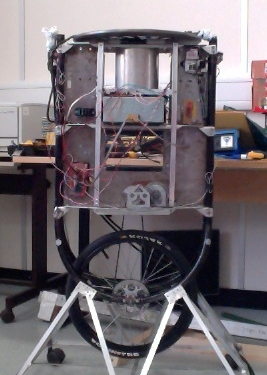
\includegraphics[width=\linewidth]{figures/old.jpg}
			\caption{Old, \SI{1}{\meter} tall}
			\label{fig:uni-old}
		\end{subfigure}%
		\hfill%
		\begin{subfigure}{0.3\linewidth}
			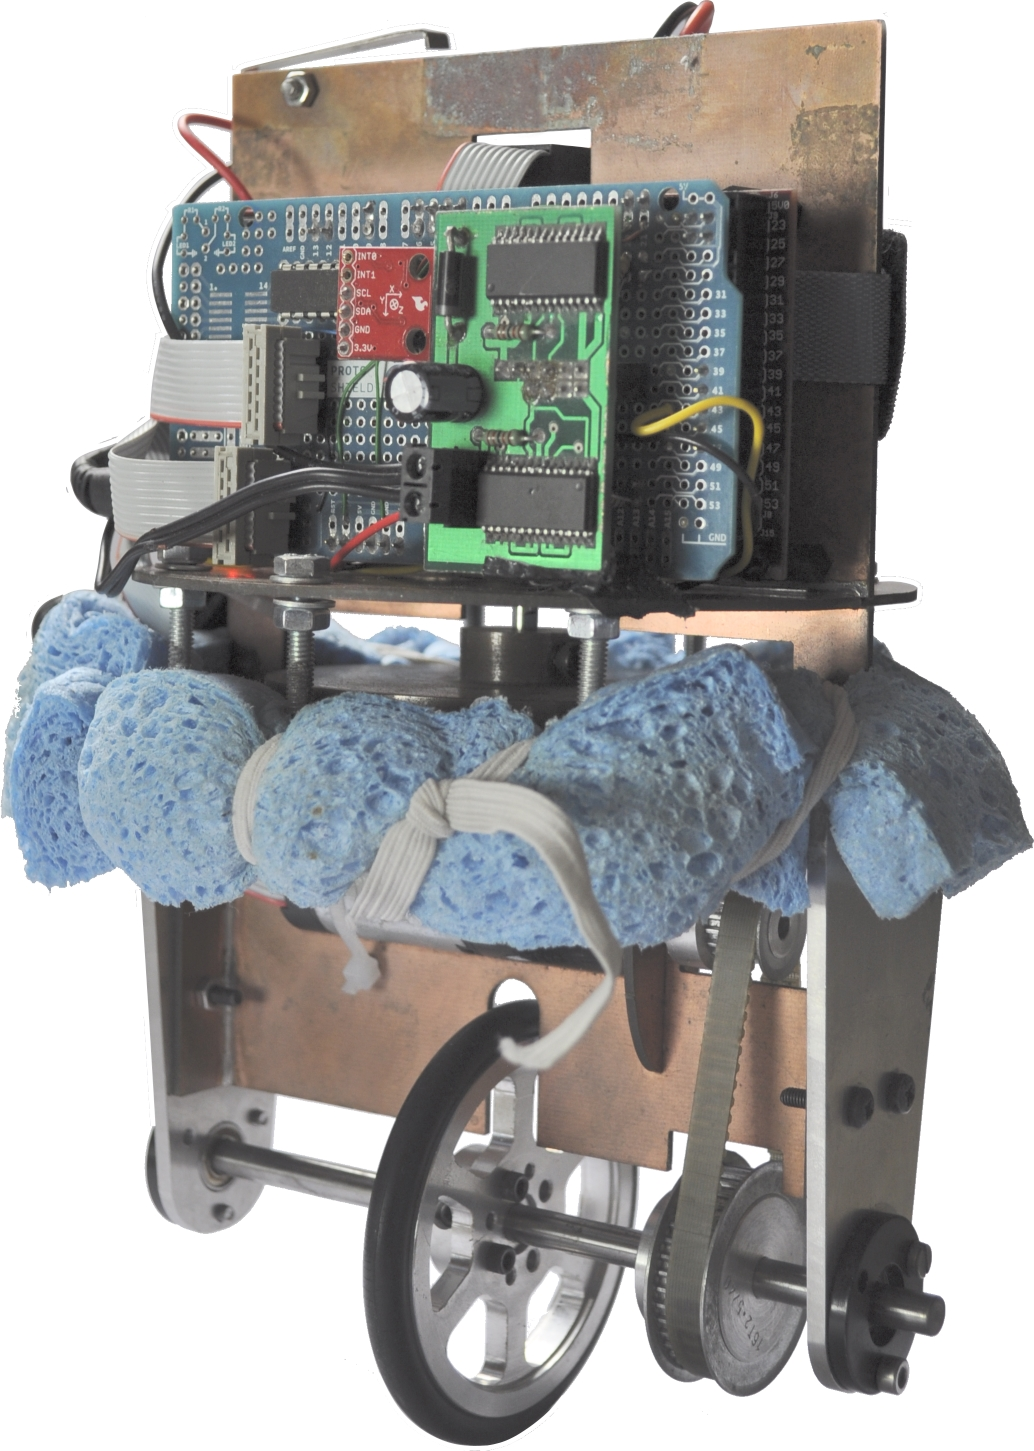
\includegraphics[width=\linewidth]{figures/front.jpg}
			\caption{New, \SI{20}{\centi\meter} tall}
			\label{fig:uni-new}
		\end{subfigure}
		\hspace*{\fill}
		\caption{Unicycle robot configurations}
	\end{figure}

	There is a history of unicycle robots in the Engineering Department dating back to 2005, which is described in more detail by~\citeauthor{queiro}~\cite{queiro}.
	Alongside work on these, the \textsc{Pilco} method has been successfully applied to computer models of these unicycles ~\cite[section~3.3]{pilco}.
	Based on the work in 2011, the decision was made to move from the large and dangerous platform described there (\cref{fig:uni-old}) to a much smaller and safer model (\cref{fig:uni-new}).
	Since then, work by~\citeauthor{aleksi}~\cite{aleksi} went on to write the embedded software for the system, and performed experiments to try and reproduce the results of \textsc{Pilco} in simulation in hardware.


	This work met mixed success -- many problems in the hardware were identified and fixed, and there was some evidence of learning, with the controller marginally improving over time.
	However, various concerns were raised with the testing procedure, and the computer model of the unicycle was never updated to match the hardware -- making it difficult to judge whether problems lay in the hardware or in simply a more difficult control task than on the larger unicycle, and raising concerns about whether other parts of the software stack were still configured for the large robot.

	\subsection{Application of \textsc{Pilco} to the unicycle}
		For the purposes of \textsc{Pilco}, our action and reduced (ie., the components used for learning) state vectors are
		\begin{align}
			\bm{x} &= \begin{bmatrix}
				\dot\theta & \dot\phi &\dot\psi_w & \dot\psi & \dot\psi_t &
				x_c & y_c &
				\theta &
				\phi & \psi
			\end{bmatrix}^T &
			\bm{u} &= \begin{bmatrix}
				\tau_t & \tau_w
			\end{bmatrix}^T\,, \label{eq:state-vars}
		\end{align}
		where $\theta$ is the roll angle, $\phi$ is yaw, $\psi_w$ wheel angle,
		$\psi$ pitch angle, $\psi_t$ the turntable angle, and $x_c, y_c$ are the position of the world-origin in the coordinate space of the robot.
		$\tau_t$ and $\tau_w$ are the control torques on the turntable and wheel, respectively.
		In simulation, some extra states ($\dot{x}_c, \dot{y}_c, \psi_w, \psi_t$) are needed in order to implement the dynamics derived by~\citeauthor{forster}~\cite{forster}.

		In this report, we restrict our search for optimal controllers to affine controllers of the form
		$\bm{u} = \pi(\bm{x}) = W\bm{x} + \bm{b}$, and choose cost functions of the form
		$c(\bm{x}, \bm{u}) = 1 - \mathbb{E}_{\bm{x}} \exp\left[-\frac{1}{2} f(\bm{x})^T Q f(\bm{x})\right]$, where $f$ is a function that appends trigonometric functions of $\phi, \theta, \psi$ to the end of the state vector, aiding in penalization of geometric properties.

		Each GP in \cref{eq:transition-gp} modelling the dynamics of a single state is parametrized by $m$, $K$ of the form
		\begin{align}
			m(\bm{z}) &= \bm{z} \cdot \bm{w} + b \\
			K(\bm{z}_1, \bm{z}_2) &= \sigma_s^2 \exp \left(
				-\frac{1}{2}
				\bm{z}_1^T
				\begin{bmatrix}
					\bm{l}_1^2 && \\
					& \ddots & \\
					&& \bm{l}_n^2
				\end{bmatrix}^{-1}
				\bm{z}_2
			\right) + \sigma_n^2 I \,,
		\end{align}
		where $\sigma_s^2$ and $\sigma_n^2$ estimate the signal and noise variances, $\bm{w}$ (weight) and $b$ (bias) define a simple affine mean function, and $\bm{l}$ (length) defines a length-scale for the problem for each of the state variables.
		Note that these parameters have a unique value for each state.

\section{Goals and direction of this work}
	\label{sec:dry}

	Like previous work, the ideal goal of this project is to apply \textsc{Pilco} to the unicycle robot, and achieve an outcome of a successfully balancing controller.
	Previous work went to great lengths experimentally to achieve this goal, with limited success. Thankfully, this work was not wasted, as it raised and fixed mechanical and electrical problems, freeing this work from their hindrances.

	However, few problems were traced back as far as the \textsc{Pilco} software -- indeed, none of the changes made to it during~\cite{aleksi} were kept, indicating that they were at best hacks.
	One of the problems with machine learning is that it's very hard to tell the difference between failure to learn due to a hard problem or insufficiently flexible model, and failure to learn due to programmatic errors in the implementation.
	This work therefore took on an approach of critically reviewing the source code used, targeting obvious problems with non-obvious repercussions.

	In the process of reviewing source code, software engineering best-practices were kept in mind, and applied retrospectively to correct and incorrect code alike.
	A particularly important principle in software design is DRY, or \enquote{Don't Repeat Yourself}.
	More specifically, this advocates that \enquote{Every piece of knowledge must have a single, unambiguous, authoritative representation within a system}\cite{dry}.
	To see the value in holding this principle, consider a case where there are two representations. If the piece of knowledge changes, such as the mass of the robot decreasing, now two places need updating. If one of them is missed, then the result is an incorrect system. This principle applies not only to data, but also procedures.

	In addition, many of the tools were improved to streamline the process of applying \textsc{Pilco} to real hardware, most of which are transferable to other non-unicycle investigations in future.


\bib

\end{document}